\documentclass[conf]{new-aiaa}
%\documentclass[journal]{new-aiaa} for journal papers
\usepackage[utf8]{inputenc}

\usepackage{graphicx}
\usepackage{amsmath}
\usepackage[version=4]{mhchem}
\usepackage{siunitx}
\usepackage{longtable,tabularx}
\usepackage{float}
\usepackage{csvsimple}
\setlength\LTleft{0pt} 

\title{Project 2}
\author{Mauro Patimo}
\begin{document}
\maketitle

\section{Nomenclature}

{\renewcommand\arraystretch{1.0}
\noindent\begin{longtable*}{@{}l @{\quad=\quad} l@{}}
$f$  & equation introduced in similarity solution \\
$\eta$ & variable introduced in similarity solution to relate y and x\\

\end{longtable*}}

\section{Introduction}
Falkner-Skan equations are a set of nonlinear differential equations that describe the flow of a viscous, incompressible fluid over a flat plate. The equations are a generalization of the Blasius equation, which is obtained by setting the pressure gradient to zero. \\
The following paper will present a numerical solution to the Falkner-Skan equations for different values of the parameter $\beta$. \\
\section{Procedure}
The equations are:
\begin{equation}
    f'''+ff''+\beta(1-f'^2)=0
\end{equation}
With the following boundary conditions:
\begin{equation}
    f(0)=f'(0)=0, \quad f'(\infty)=1
\end{equation}

\section{Results}
\begin{figure}[H]
    \centering
    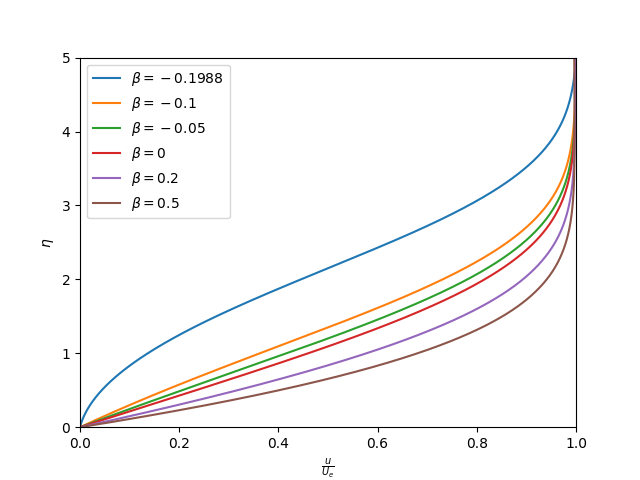
\includegraphics[width=0.5\textwidth]{Project 2.png}
    \caption{Falkner-Skan flow for different betas}
    \label{fig:Falkner-Skan for different betas}
\end{figure}

\begin{center}
    \resizebox{0.35\linewidth}{!}{\begin{tabular}{rrrr}
\hline
   $\beta$ &   $\frac{\theta}{g(x)}$ &   $c_f Re_{\theta}$ &     $H$ \\
\hline
    0.5    &                0.350299 &          0.649846   & 2.2958  \\
    0.2    &                0.408342 &          0.560824   & 2.40849 \\
    0      &                0.469342 &          0.440563   & 2.59369 \\
   -0.05   &                0.490107 &          0.392059   & 2.67814 \\
   -0.1    &                0.514655 &          0.328216   & 2.80418 \\
   -0.1988 &                0.575706 &          0.00547205 & 3.98866 \\
\hline
\end{tabular}}
\end{center}

\section{Conclusion}

\appendix
Additional work has been done to solve the Falkner-Skan equations for different values of $\beta$. 
\begin{figure}[H]
    \centering
    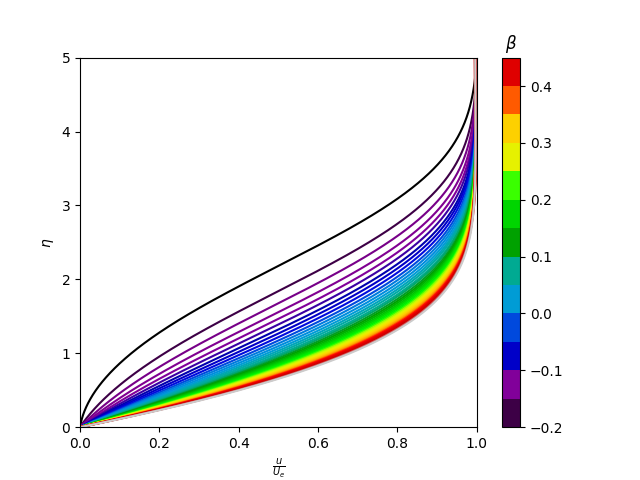
\includegraphics[width=0.5\textwidth]{Continuous beta.png}
    \caption{Falkner-Skan flow for different betas}
    \label{fig:Falkner-Skan multiples betas}
\end{figure}
\end{document}
